\documentclass[PROP_AGutteridge_CS.tex]{subfiles}
\begin{document}

\chapter{Objectives}
The aims as outlined previously will be achieved by a comprehensive approach that both processes data and presents it in an alternative style. NED will be ameliorated by combining bibliographic data with geographical and semantic information from services external to PubMed. To improve the user's search experience, a visual and interactive user interface will be created from these newly informative data, allowing the user to explore citations relative to a topic of interest or the location and institutions. This system will be available as a web application that is compatible with modern browsers. The key objectives are comprised of the modular components of the app, namely:
\begin{itemize}
\item{Implementation of a web framework}
\item{Retrieval and manipulation of data from NCBI}
\item{Semantic categorisation of keywords}
\item{Visualisation of results within a web browser} 
\end{itemize}

\section{Proposed System Architecture}
The outline of the system as proposed in the objectives can be organised to create a web application with a server-side for retrieval and processing of results from PubMed, and a client-side for visualisation of the results. 

\begin{wrapfigure}{r}{0.5\textwidth}
	\begin{center}
	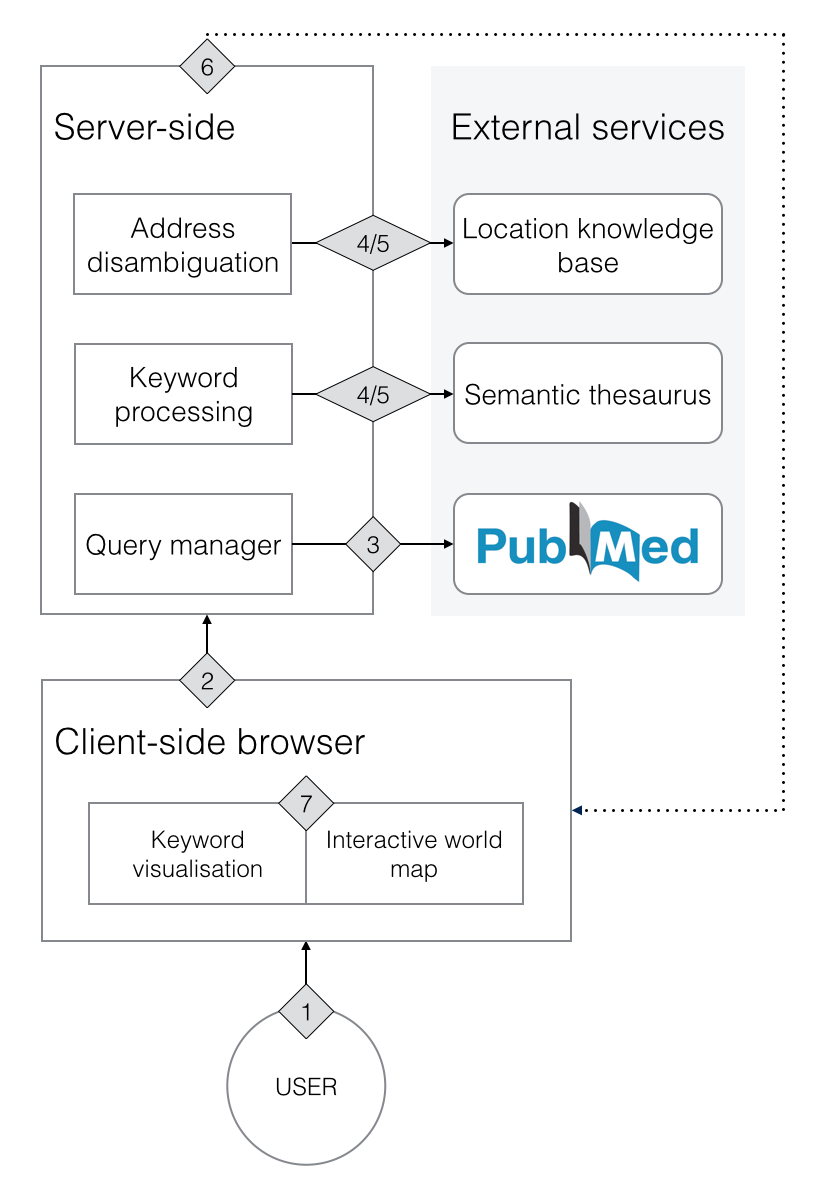
\includegraphics[width=\textwidth]{../lib/images/system-arch}
	\label{fig:SA}
  	\end{center}
 	\caption{High-level flow diagram of architecture components and structure. 1. The user interacts with the web application. 2. This sends the query to the server, 3. which sends a GET request to the PubMed database and retrieves the results in XML or JSON format, 4/5. These two stages are interchangeable, as they deal with different kinds of data. Keyword processing will be carried out on the MeSH term and author keyword }
\end{wrapfigure}

\section{Programming Languages and Web frameworks}
\subsection{Python vs. Ruby}
NCBI allows public access to the Entrez databases via the E-utilities (or eUtils) API, which follows a RESTful architecture structure. Sending HTTP requests can be easily achieved in a variety of programming languages. I have chosen to focus on dynamic programming languages as these allow for fast iterative development, which is particularly useful for web applications. I am familiar with Python and Ruby, and each have a multitude of full-stack frameworks and microframeworks to choose from. Python provides comprehensive functionality with modules for sending HTTP requests (urllib and httplib in Python 2, or urllib.request/urllib.parse/urllib.error and http.client in Python 3) and parsing XML (xml.etree.ElementTree) in the standard library. Ruby has modules for HTTP requests, but XML handling requires additional software. Despite having basic knowledge of Ruby, I am keen to learn Python and feel that overall, it is better suited for the task. 

\subsection{Flask vs. Bottle}
At this stage of the project I am unsure of the requirement for large-scale persistence of data, in which case it may be best to go forward with a microframework. This will allow for flexibility when evaluating database technologies throughout development, as full-stack frameworks such as Django require a database engine for certain features. Two microframeworks of interest are Flask (\url{http://flask.pocoo.org/}) and Bottle (\url{http://bottlepy.org/}), both of which are lightweight, supportive of RESTful APIs, and well-documented. Considering that this project is my first experience in web development, extensive documentation is a priority for choosing a framework, and an active community is also preferred. Searching for questions tagged with 'bottle' or 'flask' on StackOverflow produced 786 and 7,387 results, respectively, indicating that Flask is more popular and thus will be better supported on forums and other online communities. For this reason Flask is chosen as the most appropriate microframework with which to build the server-side of the application.\\

\section{Semantic Analysis Tools} 
\subsection{ARIANA}

\section{Address Disambiguation}
address disambiguation hopefully going to be sorted by Google Places! Considered OSM but location information/disambiguation not as good (ref that?). 


\section{Visualisation Libraries}
\subsection{Why JavaScript?} 
   
 
\end{document}